\documentclass[10pt,a4paper]{report}
\usepackage[utf8]{inputenc}
\usepackage[english]{babel}
\usepackage{amsmath}
\usepackage{amsfonts}
\usepackage{amssymb}
\usepackage{graphicx}
\usepackage[left=2cm,right=2cm,top=2cm,bottom=2cm]{geometry}
\author{Daniele Gilio}
\title{Spoken Digits Recognition}
\begin{document}
\maketitle
\section{Introduction}
This assignment is about spoken digits recognition. The dataset is comprised of $1760$ training samples, $120$ validation samples and $120$ test samples. The dataset has already been processed so that each sample represents the spectrogram of a given digit. Spectrograms are visual representation of audio, the power of the recorded sound wave is divided between $16$ frequencies and $64$ time periods creating images like the one in Figure \ref{fig:data_spect}. Our objective is to create a Neural Network (a Multi-Layer Perceptron to be precise) in order to recognize the spoken digits.
\begin{figure}[!ht]
\centering
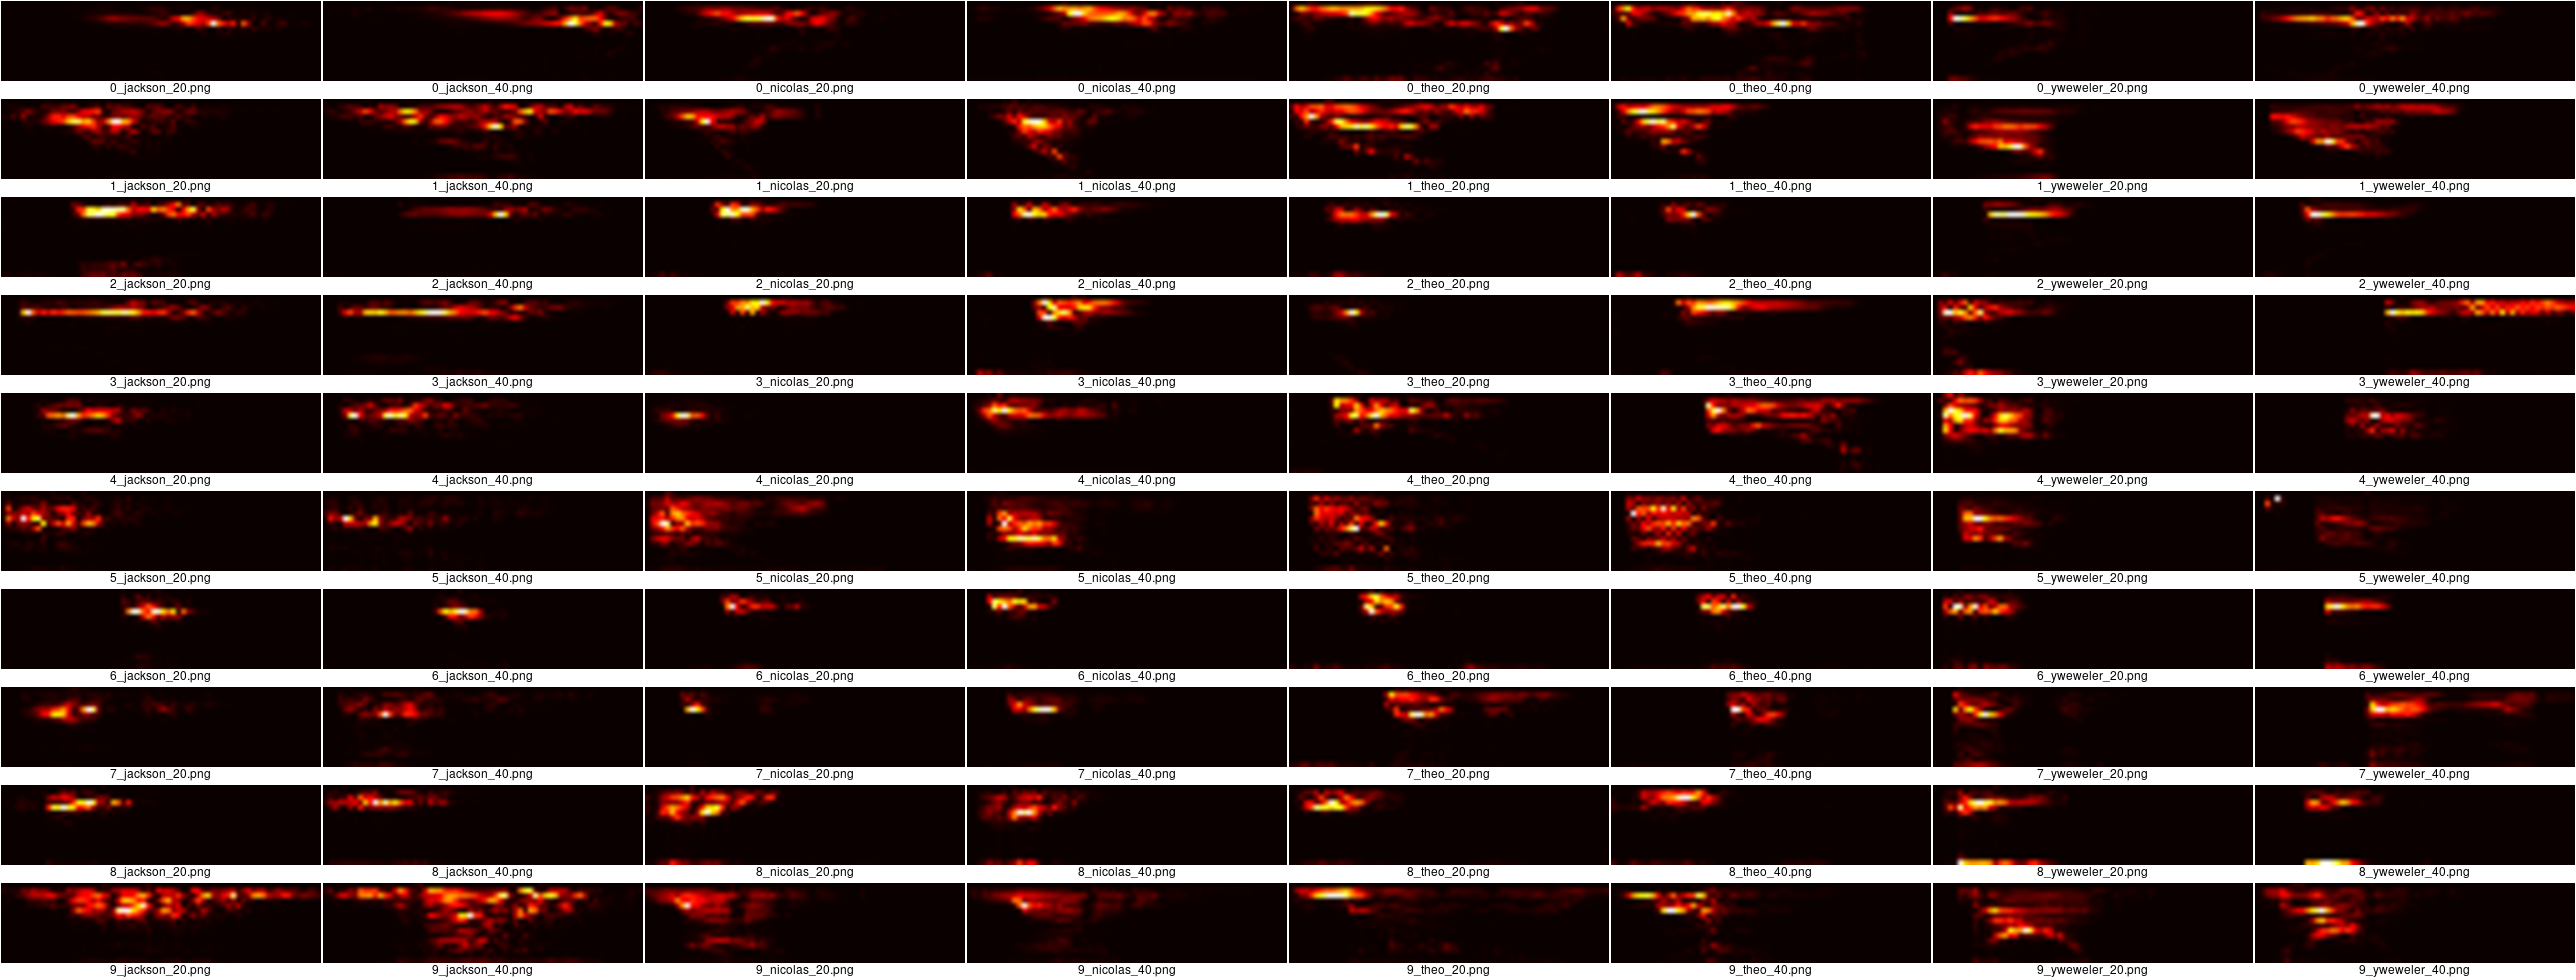
\includegraphics[width=\linewidth]{spoken-digits/spectrograms.png}
\caption{Example of the dataset spectrograms}
\label{fig:data_spect}
\end{figure}
\section{Data Visualization and Analysis}
In order to test our code we plotted spectrograms after we loaded the data and after performing normalization. The second plotting was also done in order to verify that the normalization did not interfere too much with the data. At this stage we opted for an L2 Normalization sine we feel that, since the data in a single vector are probably strongly correlated, avoiding statistic normalization might be a feasible choice. We can see the output of our code in Figure ().
\section{Neural Network}
In order to experiment a bit with Neural Networks we built a Single-Layer Perceptron in which we have only an input layer and an output layer. As in the previous assignment we implemented a varying learning rate.
\subsection{Architecture}
After playing a bit with network architectures we settled on the following sequence $[1024, 256, 128, 32, 10]$, representing the width of each layer. Bigger models tended to overfit and took a long time to train, on the other hand tinier models were faster to train but less precise. We believe that optimal values are not very far from the ones we found.
\subsection{Hyperparameters and Training}
In order to train our network we tested Gradient Descent, SGD and mini-batch SGD. The first one proved to be the smoothest but the slowest and hardware demanding, SGD was the fastest but the most erratic. Mini-batch SGD was a good compromise between the two, we choose a batch size of $8$ so to exploit the full capabilities of our hardware. The number of steps was adjusted accordingly to the batch size. 
\subsection{Normalization Techniques}
\section{Results}
\section{Conclusions}
\end{document}